\subsection{Class Diagram}
\begin{figure}[H]
	The picture below shows the class digram of Lunar Rover project. There 4 main important classes in this project:
	\begin{itemize}
		\item AppStateRepository class hold all data imported/collected in application
		\item RobotConnectionSerivce and RobotMovementService responsible for connecting and control movement of robot.
		\item ServiceManager responsible for managing services use in application
		\item StateMachineBuilder responsible for controlling and switching between states of robot.
	\end{itemize}
	\centering
	\hspace*{-25mm}
	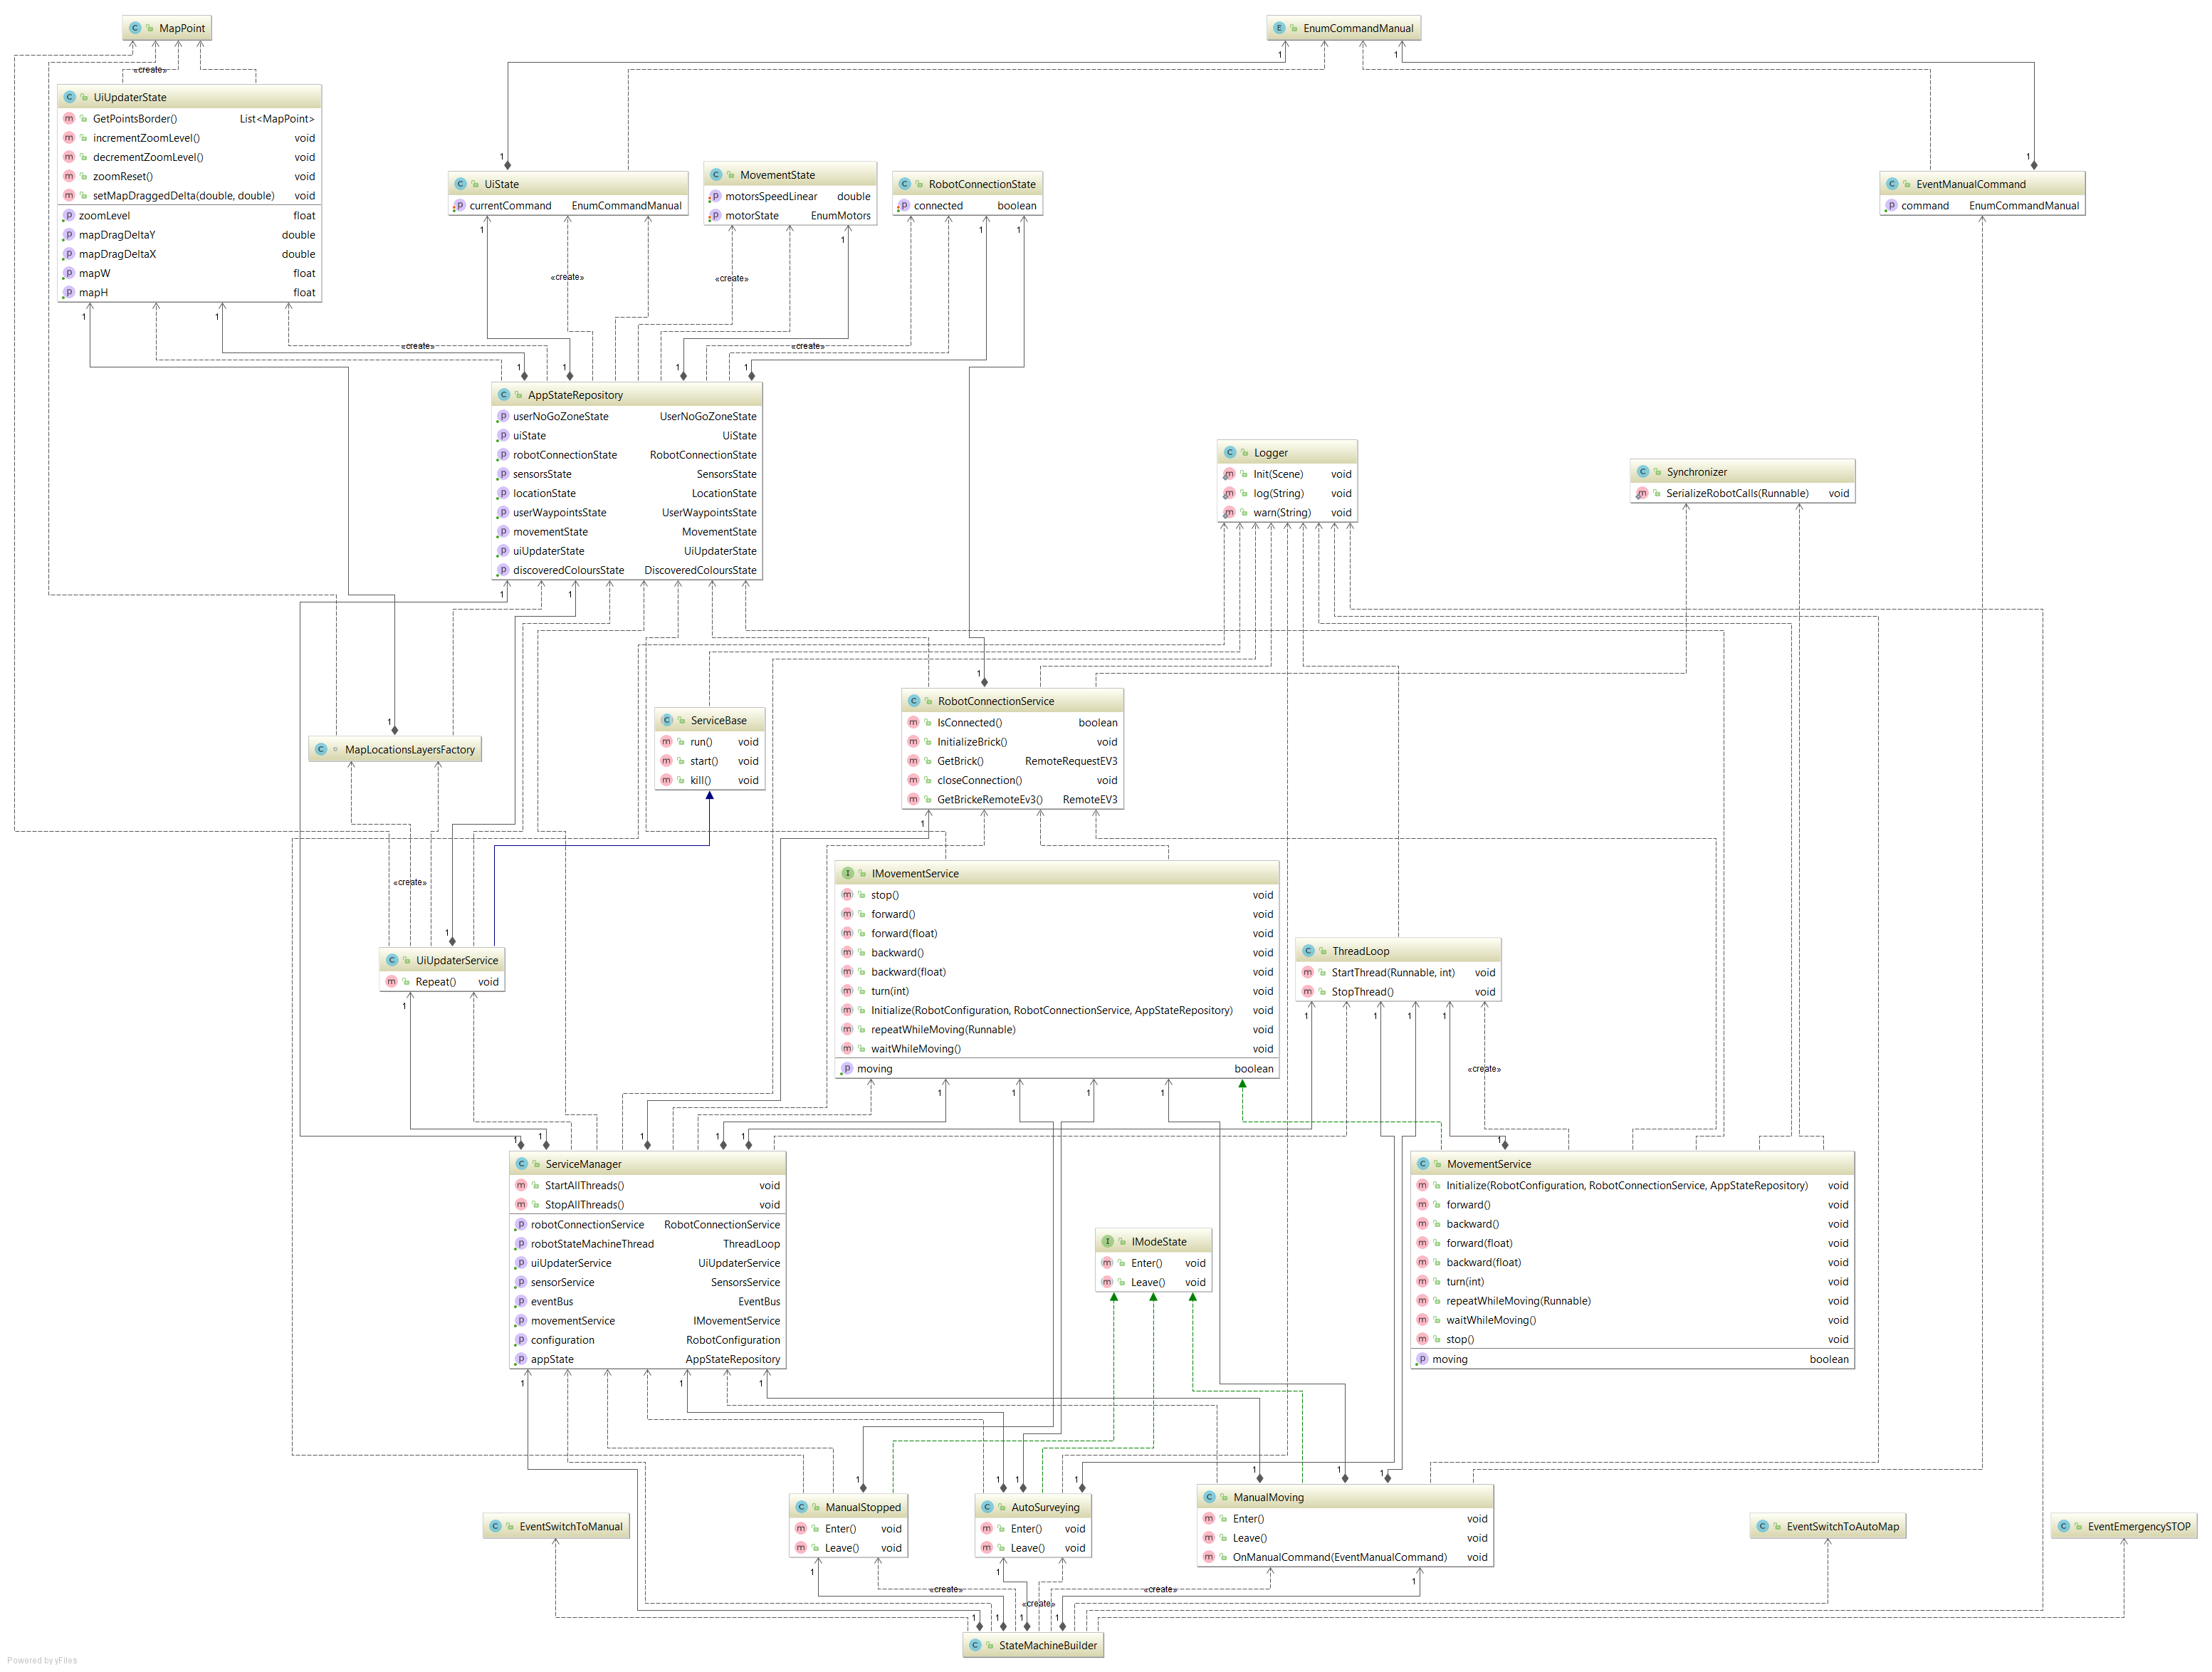
\includegraphics[width=1.4\textwidth]{ClassDiagram.png}	
	\caption{\label{fig:diagramClasses}Class diagram of the whole system}
\end{figure}	

\subsection{State Diagram}
\begin{figure}[H]
	The picture below shows the state diagram of Lunar Rover project. There three main states:
	\begin{itemize}
		\item Auto survey state is the state when robot autonomous moving and survey the map.
		\item Manual control state is the state when robot will move under control of user.
		\item Idle state is when robot is stop moving.
	\end{itemize}
	\centering
	\hspace*{-15mm}
	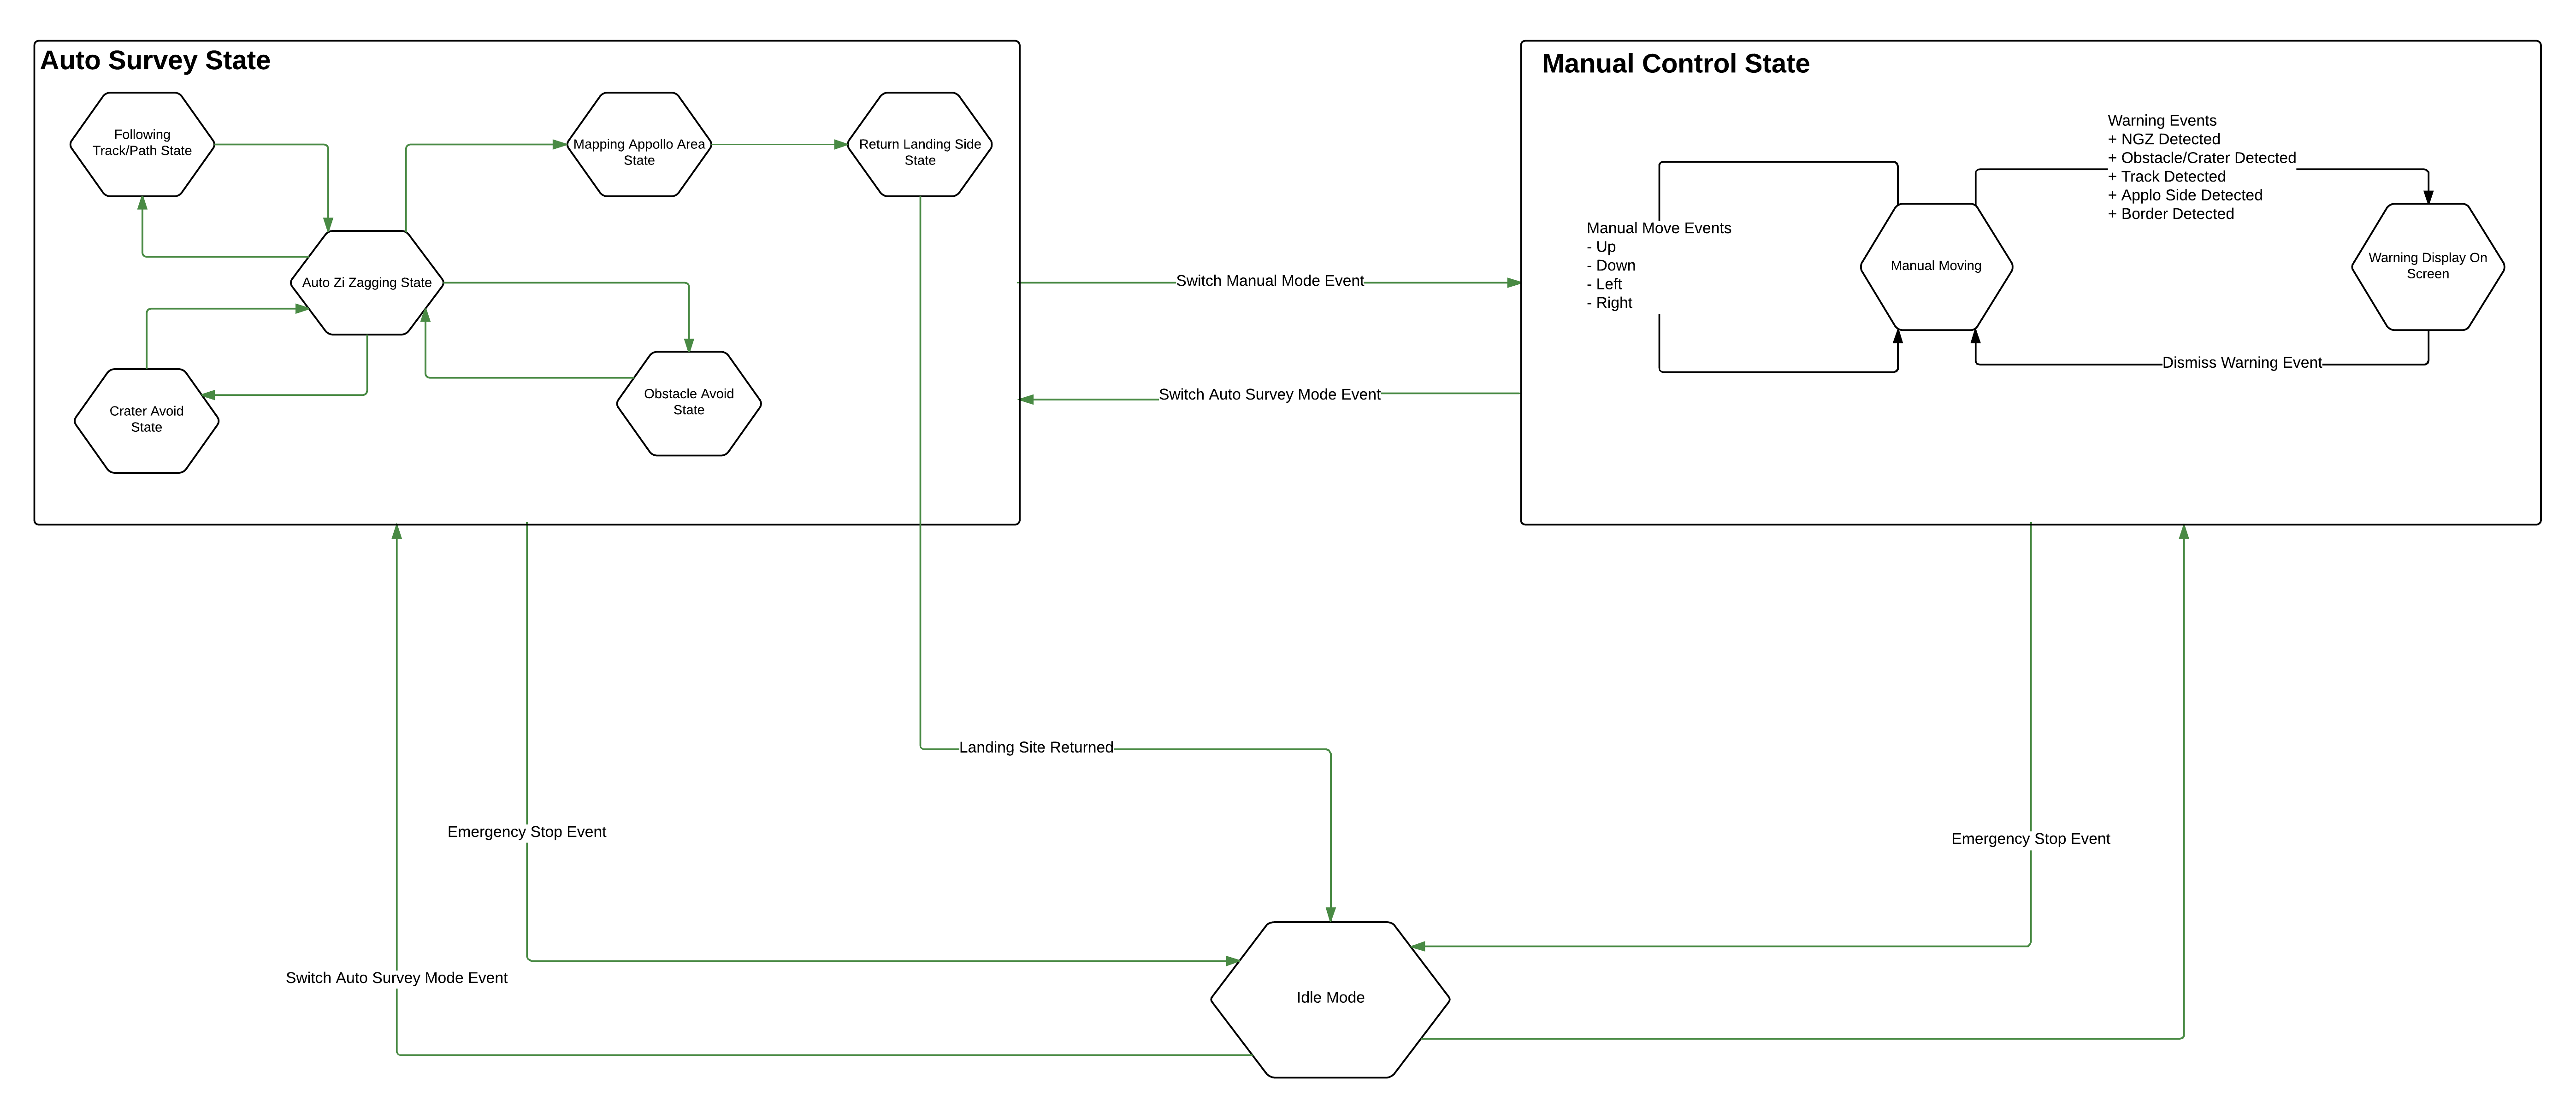
\includegraphics[width=1.2\textwidth]{StateDiagram.png}	
	\caption{\label{fig:diagramState}The State Diagram of the whole system}
\end{figure}	

\subsection{Interaction Diagram}
The picutre below shows the integration diagram of Lunar Rover system.
\begin{figure}[H]
	\centering
	\hspace*{-25mm}
	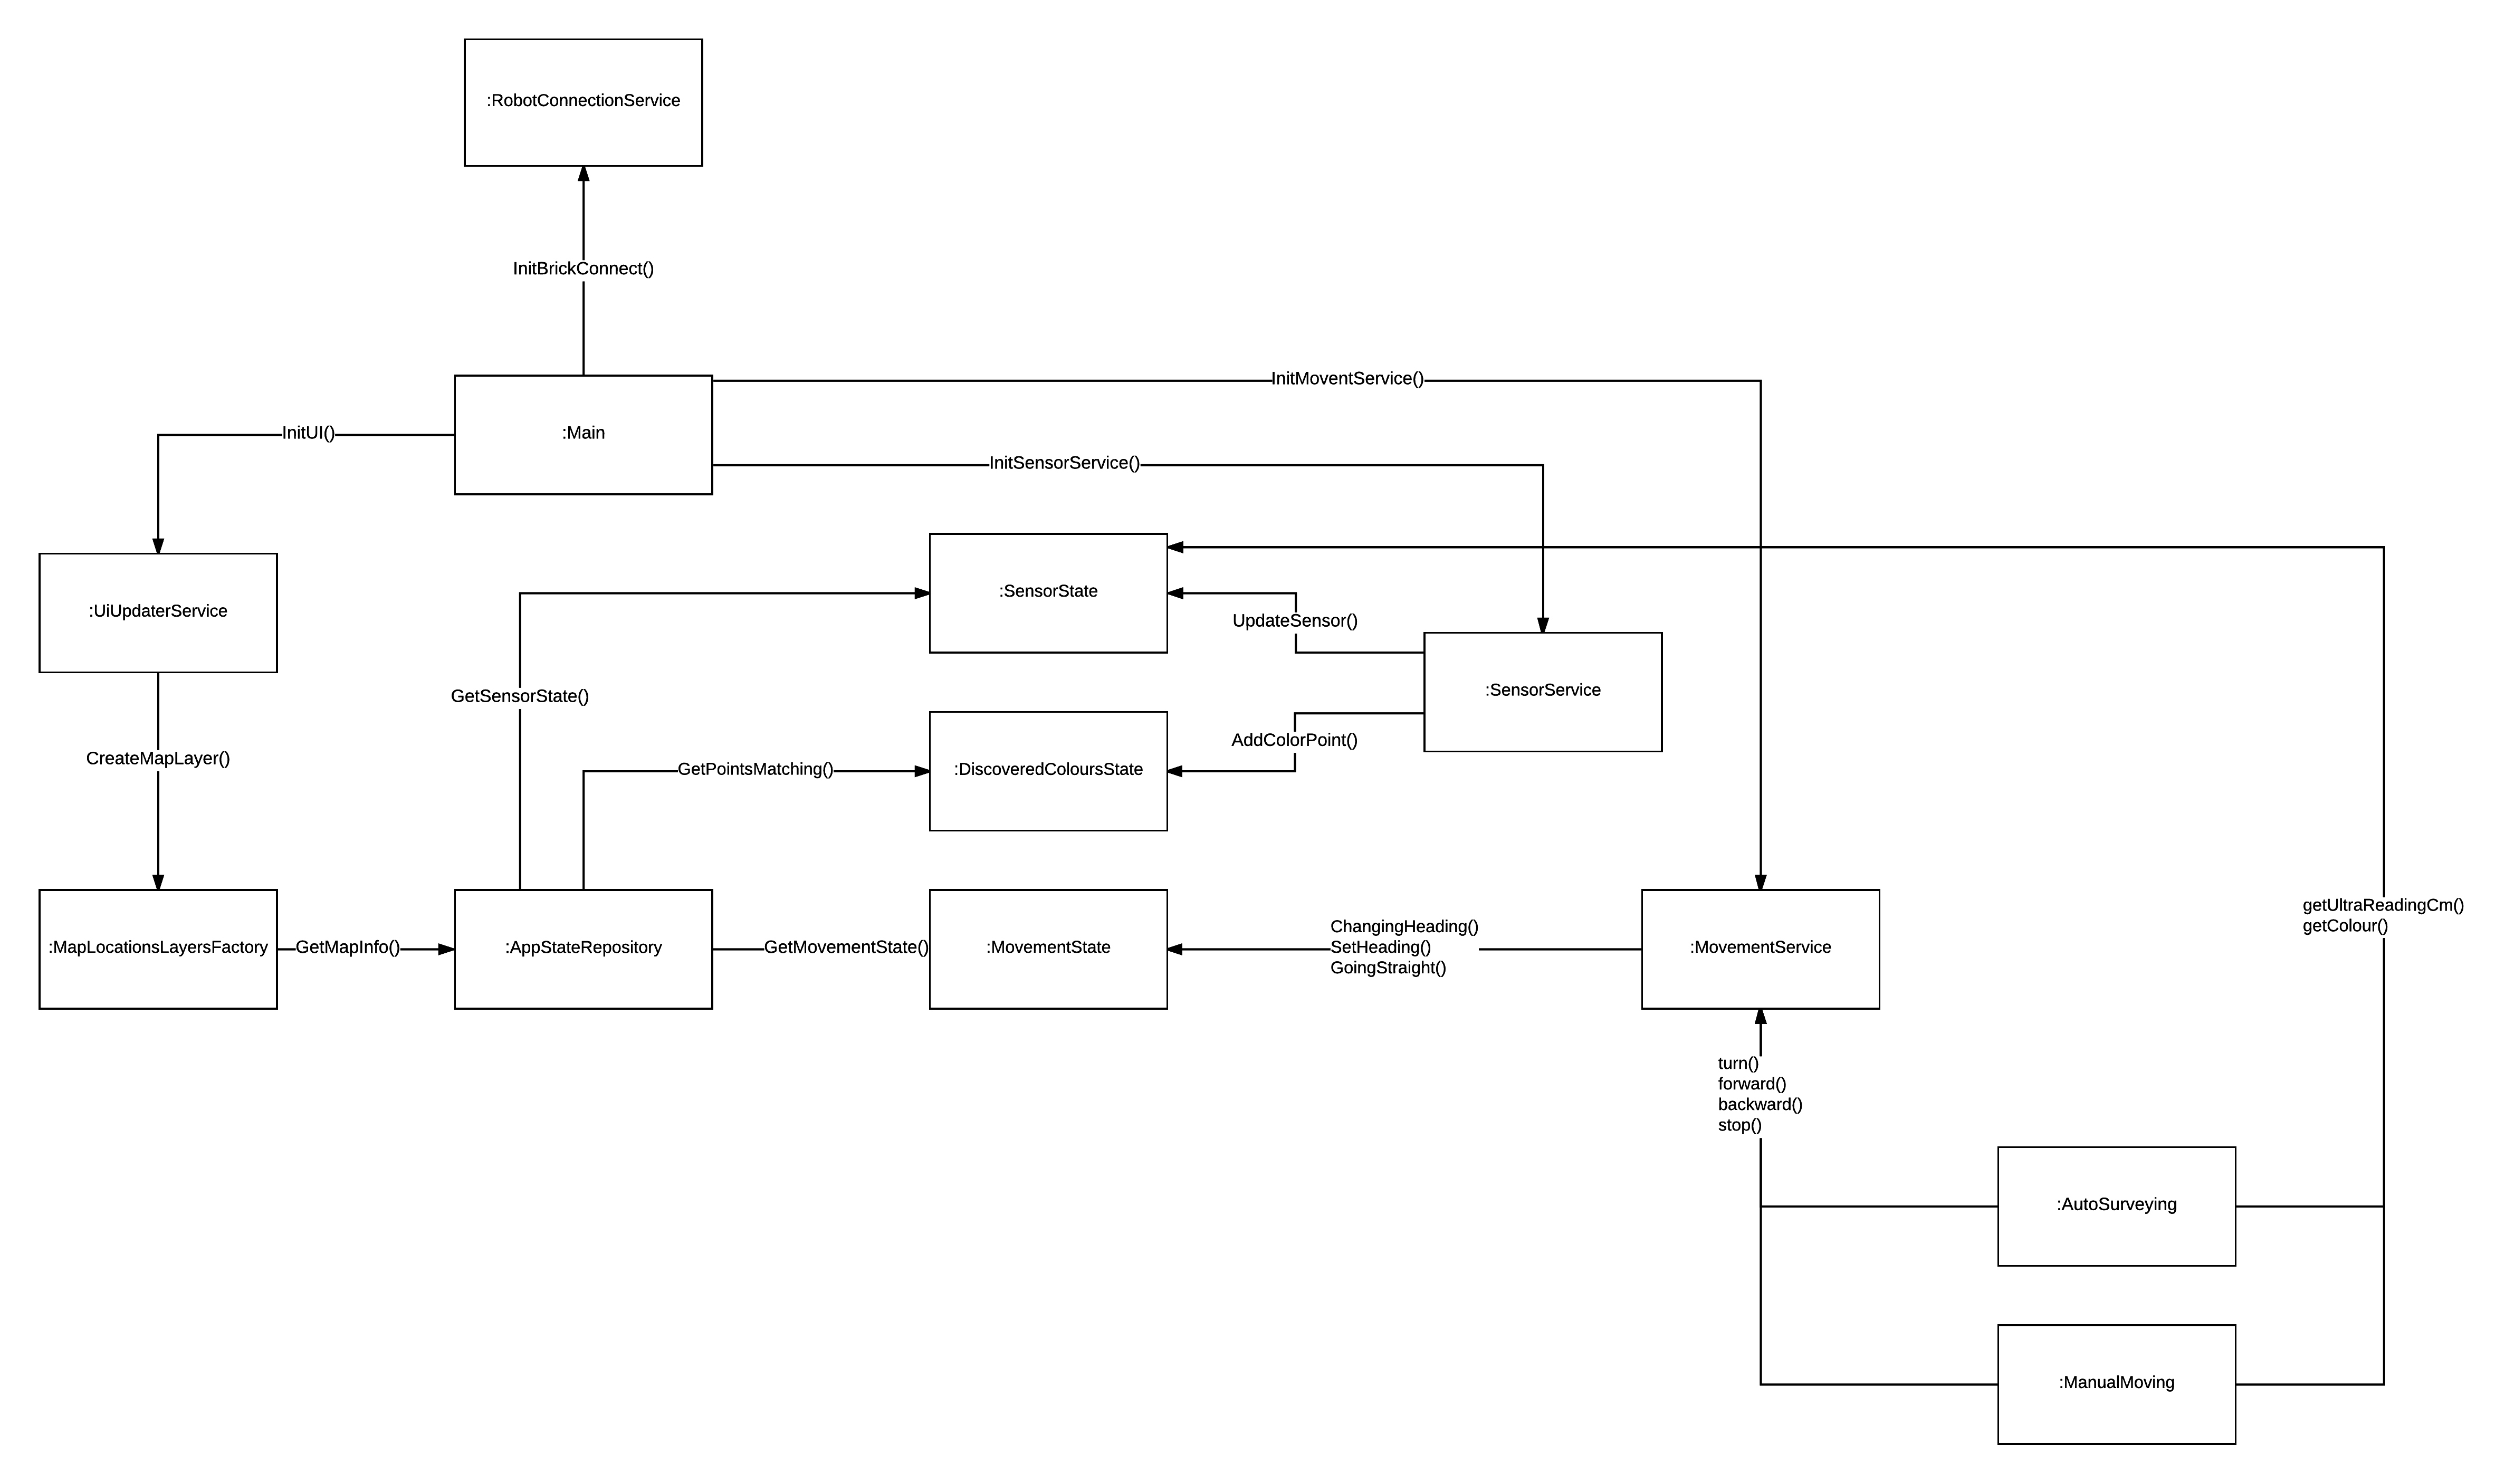
\includegraphics[width=1.4\textwidth]{InteractionDiagram.png}	
	\caption{\label{fig:diagramInteraction}The interaction diagram of the whole system}
\end{figure}	